% %% %%%%%%%%%%%%%%%%%%%%%%%%%%%%%%%%%%%%%%%%%%%%%%%%%%%%%%%%%%
% practica.tex
%
% Author:  Mauricio Matamoros
% License: MIT
%
% %% %%%%%%%%%%%%%%%%%%%%%%%%%%%%%%%%%%%%%%%%%%%%%%%%%%%%%%%%%%

% CHKTEX-FILE 1
\documentclass[letterpaper,10.5pt]{article}
% %% %%%%%%%%%%%%%%%%%%%%%%%%%%%%%%%%%%%%%%%%%%%%%%%%%%%%%%%%%
%
% packages.tex
%
%  Author: Mauricio Matamoros
%  Date:   2020.02.28
%
%  Contiene la lista de paquetes requeridos para generar
%  el archivo-reporte de las prácticas de laboratorio
%
% %% %%%%%%%%%%%%%%%%%%%%%%%%%%%%%%%%%%%%%%%%%%%%%%%%%%%%%%%%%
% Archivo principal de LaTeX
%!TEX root = ../reporte.tex

\usepackage[utf8]{inputenc}                  % Soporte para utf8
\usepackage[T1]{fontenc}                     % Soporte extendido de caracteres unicode
\usepackage[english,spanish,mexico]{babel}   % Define el idioma del documento a español (México) con soporte para inglés
% Standard packages
\usepackage{float}                           % Imágenes flotantes en el documento
\usepackage{ifthen}                          % Soporte if-then en macros
\usepackage{xspace}                          % Soporte de autoespaciado en macros
\usepackage{xstring}                         % Operaciones con cadenas en macros
\usepackage{wrapfig}                         % Permite colocar texto al rededor de figuras y otros flotantes
\usepackage{booktabs}                        % Embellece tablas
\usepackage{csquotes}                        % Entrecomillado automático y manejo de citas textuales
\usepackage{fancyhdr}                        % Permite reconfigurar encabezado y pie de página
\usepackage{fancyvrb}                        % Define estilos para entornos Verbatim
\usepackage{geometry}                        % Permite reconfigurar la geometría del documento
\usepackage{graphicx}                        % Permite insertar imágenes en varios formatos
\usepackage{lastpage}                        % Referencia a la última página del documento
\usepackage{listings}                        % Define estilos para entornos de código de programación (sintaxis)
\usepackage{multicol}                        % Manejo de texto en varias columnas
\usepackage{tabularx}                        % Tablas con ancho de columna variable
\usepackage{algorithm}                       % Entorno para escribir algoritmos
\usepackage{algpseudocode}                   % Entorno para escribir algoritmos en pseudocódigo
\usepackage[justification=centering]{subcaption} % Permite imágenes en viñetas
\usepackage[all]{nowidow}                    % Control de viudas y huérfanas
\usepackage[inline]{enumitem}                % Añade opciones de configuración a listas
\usepackage[usenames,dvipsnames]{xcolor}     % Permite el uso de colores en el documento
% Referencing
\usepackage{varioref}                        % Gestión de referencias variables
\usepackage{hyperref}                        % Gestión de referencias e hipervínculos
\usepackage[noabbrev,nameinlink,spanish]{cleveref} % Gestión de referencias cruzadas inteligentes con hipervínculos
\usepackage[square, comma, numbers, sort&compress]{natbib} % Gestión de referencias bibliográficas


\newcommand{\lpar}{(}\newcommand{\rpar}{)} %CHKTEX 9
\newcommand{\IIC}{I\textsuperscript{2}C\xspace}
\newcommand{\GND}{\textsc{Gnd}\xspace}
\newcommand{\VCC}{\textsc{Vcc}\xspace}
\newcommand{\VDD}{\textsc{Vdd}\xspace}
\newcommand{\textbi}[1]{\textbf{\textit{#1}}}
\newcommand{\degreesC}[1]{%
	#1\textsuperscript{o}C\xspace{}%
}
\newcommand{\degreesF}[1]{%
	#1\textsuperscript{o}F\xspace{}%
}

% \newcommand{\VCC}{V\textsubscript{CC}\xspace{}}
% \newcommand{\GND}{\textsc{Gnd}\xspace{}}
% CHKTEX-FILE 26
% CHKTEX-FILE 36

\tcbuselibrary{most}
% \tcbuselibrary{listings,breakable}
% \usetikzlibrary{shadings,shadows}
% \usetikzlibrary{decorations.pathmorphing}
% \usetikzlibrary{patterns}
% \usetikzlibrary{spy}
% \usetikzlibrary{arrows.meta}

\newtcolorbox{importantbox}[1]{%
	enhanced,
	colback=red!5!white,%
	colframe=red!75!black,%
	fonttitle=\bfseries,%
	center title,
	title={#1},%
	drop fuzzy shadow
}


\newtcolorbox{greenbox}[1]{%
	enhanced,
	colback=Green!5!white,%
	colframe=Green!75!black,%
	fonttitle=\bfseries,%
	center title,
	title={#1},%
	drop fuzzy shadow
}

\newtcolorbox{marker}[1][]{%
	enhanced,
	before skip=2mm,after skip=3mm,
	boxrule=0.4pt,left=5mm,right=2mm,top=1mm,bottom=1mm,
	colback=yellow!50,
	colframe=yellow!20!black,
	sharp corners,rounded corners=southeast,arc is angular,arc=3mm,
%	underlay={%
%		\path[fill=tcbcolback!80!black] ([yshift=3mm]interior.south east)--++(-0.4,-0.1)--++(0.1,-0.2);
%		\path[draw=tcbcolframe,shorten <=-0.05mm,shorten >=-0.05mm] ([yshift=3mm]interior.south east)--++(-0.4,-0.1)--++(0.1,-0.2);
%		\path[fill=yellow!50!black,draw=none] (interior.south west) rectangle node[white]{\Huge\bfseries !} ([xshift=4mm]interior.north west);
%	},
	drop fuzzy shadow,#1
}

%CHKTEX-FILE 1
%CHKTEX-FILE 7
%CHKTEX-FILE 9
% Default fixed font does not support bold face
\DeclareFixedFont{\ttb}{T1}{txtt}{bx}{n}{8} % for bold
\DeclareFixedFont{\ttm}{T1}{txtt}{m}{n}{8}  % for normal

% Custom colors
\usepackage{color}
\definecolor{keywordsColor}{rgb}{0,0,0.5}
\definecolor{customColor}{rgb}{0.6,0,0}
\definecolor{stringColor}{rgb}{0,0.5,0}

% Code highlighting python
\renewcommand{\ttdefault}{pcr}
\lstset{
	language=Python,                              % the language of the code (can be overrided per snippet)
	backgroundcolor=\color{white},                % choose the background color
	basicstyle=\footnotesize\ttfamily,            % the size of the fonts that are used for the code
	breakatwhitespace=false,                      % sets if automatic breaks should only happen at whitespace
	breaklines=true,                              % sets automatic line breaking
	captionpos=t,                                 % sets the caption-position to bottom
	commentstyle=\color{gray},                    % comment style
	deletekeywords={},                            % if you want to delete keywords from the given language
%	escapeinside={\%*}{*)},                       % if you want to add LaTeX within your code
	extendedchars=true,                           % lets you use non-ASCII characters; for 8-bits encodings only, does not work with UTF-8
	frame=tb,                                     % adds a frame around the code
	keepspaces=true,                              % keeps spaces in text, useful for keeping indentation of code (possibly needs columns=flexible)
	keywordstyle=\color{keywordsColor}\bfseries,  % keyword style
	numbers=left,                                 % where to put the line-numbers; possible values are (none, left, right)
	numbersep=5pt,                                % how far the line-numbers are from the code
	numberstyle=\tiny\color{gray},                % the style that is used for the line-numbers
	rulecolor=\color{black},                      % if not set, the frame-color may be changed on line-breaks within not-black text (e.g. comments (green here))
	showspaces=false,                             % show spaces everywhere adding particular underscores; it overrides 'showstringspaces'
	showstringspaces=false,                       % underline spaces within strings only
	showtabs=false,                               % show tabs within strings adding particular underscores
	stepnumber=1,                                 % the step between two line-numbers. If it's 1, each line will be numbered
	stringstyle=\color{stringColor},              % string literal style
	tabsize=2,                                    % sets default tabsize to 2 spaces
	title=\lstname,                               % show the filename of files included with \lstinputlisting; also try caption instead of title
	columns=fixed,                                % Using fixed column width (for e.g. nice alignment)
	otherkeywords={self},                         % if you want to add more keywords to the set
	emphstyle=\color{customColor}\bfseries,       % Custom highlighting style
	emph={__init__,__main__,True,False,None},     % Custom highlighting keywords
	xleftmargin=1cm,                              % Left margin
	xrightmargin=1cm,                             % Right margin
	% Unicode compatibility
	inputencoding=utf8,
	literate={%
	            {Á}{{\'a}}1 {É}{{\'E}}1 {Í}{{\'I}}1 {Ó}{{\'O}}1 {Ú}{{\'U}}1%
	            {á}{{\'a}}1 {é}{{\'e}}1 {í}{{\'i}}1 {ó}{{\'o}}1 {ú}{{\'u}}1%
	            {À}{{\`A}}1 {È}{{\'E}}1 {Ì}{{\`I}}1 {Ò}{{\`O}}1 {Ù}{{\`U}}1%
	            {à}{{\`a}}1 {è}{{\`e}}1 {ì}{{\`i}}1 {ò}{{\`o}}1 {ù}{{\`u}}1%
	            {Ä}{{\"A}}1 {Ë}{{\"E}}1 {Ï}{{\"I}}1 {Ö}{{\"O}}1 {Ü}{{\"U}}1%
	            {ä}{{\"a}}1 {ë}{{\"e}}1 {ï}{{\"i}}1 {ö}{{\"o}}1 {ü}{{\"u}}1%
	            {Â}{{\^A}}1 {Ê}{{\^E}}1 {Î}{{\^I}}1 {Ô}{{\^O}}1 {Û}{{\^U}}1%
	            {â}{{\^a}}1 {ê}{{\^e}}1 {î}{{\^i}}1 {ô}{{\^o}}1 {û}{{\^u}}1% CHKTEX 19
	            {Ã}{{\~a}}1 {Ẽ}{{\~E}}1 {Ĩ}{{\~I}}1 {Õ}{{\~O}}1 {Ũ}{{\~U}}1 {Ñ}{{\~N}}1%
	            {ã}{{\~a}}1 {ẽ}{{\~e}}1 {ĩ}{{\~i}}1 {õ}{{\~o}}1 {ũ}{{\~u}}1 {ñ}{{\~n}}1%
	            {œ}{{\oe}}1 {Œ}{{\OE}}1 {æ}{{\ae}}1 {Æ}{{\AE}}1 {ß}{{\ss}}1%
	            {ç}{{\c c}}1 {Ç}{{\c C}}1 {ø}{{\o}}1 {å}{{\r a}}1 {Å}{{\r A}}1%
	            {€}{{\EUR}}1 {£}{{\pounds}}1 {×}{{\(\times\)}}1% CHKTEX 21
	            {°}{{\textsuperscript{o}}}1%
	            {¹}{{\textsuperscript{1}}}1%
	            {²}{{\textsuperscript{2}}}1%
	            {³}{{\textsuperscript{3}}}1%
	            {⁴}{{\textsuperscript{4}}}1% CHKTEX 19
	            {⁵}{{\textsuperscript{5}}}1% CHKTEX 19
	            {⁶}{{\textsuperscript{6}}}1% CHKTEX 19
	            {⁷}{{\textsuperscript{7}}}1% CHKTEX 19
	            {⁸}{{\textsuperscript{8}}}1% CHKTEX 19
	            {⁹}{{\textsuperscript{9}}}1% CHKTEX 19
	            {⁰}{{\textsuperscript{0}}}1% CHKTEX 19
%	            {A}{{\textAlpha}}1
	            {α}{{\textalpha}}1%
%	            {B}{{\textBeta}}1
	            {β}{{\textbeta}}1%
	            {Γ}{{\textGamma}}1
	            {γ}{{\textgamma}}1%
	            {Δ}{{\textDelta}}1
	            {δ}{{\textdelta}}1% CHKTEX 19
%	            {E}{{\textEpsilon}}1
	            {ϵ}{{\textepsilon}}1%
%	            {Z}{{\textZeta}}1
	            {ζ}{{\textzeta}}1%
%	            {H}{{\textEta}}1
	            {η}{{\texteta}}1%
	            {Θ}{{\textTheta}}1
	            {θ}{{\texttheta}}1%
%	            {I}{{\textIota}}1
	            {ι}{{\textiota}}1%
%	            {K}{{\textKappa}}1
	            {κ}{{\textkappa}}1%
	            {Λ}{{\textLambda}}1
	            {λ}{{\textlambda}}1%
%	            {M}{{\textMu}}1
	            {μ}{{\textmu}}1%
%	            {N}{{\textNu}}1
	            {ν}{{\textnu}}1%
	            {Ξ}{{\textXi}}1
	            {ξ}{{\textxi}}1%
%	            {O}{{\textOmikron}}1
%	            {o}{{\textomikron}}1%
	            {Π}{{\textPi}}1
	            {π}{{\textpi}}1%
%	            {P}{{\textRho}}1
	            {ρ}{{\textrho}}1%
	            {Σ}{{\textSigma}}1
	            {σ}{{\textsigma}}1%
%	            {T}{{\textTau}}1
	            {τ}{{\texttau}}1%
	            {ϒ}{{\textUpsilon}}1
	            {υ}{{\textupsilon}}1%
	            {Φ}{{\textPhi}}1
	            {ϕ}{{\textphi}}1%
%	            {X}{{\textChi}}1
	            {χ}{{\textchi}}1%
	            {Ψ}{{\textPsi}}1
	            {ψ}{{\textpsi}}1%
	            {Ω}{{\textOmega}}1
	            {ω}{{\textomega}}1%
	            {ζ}{{\varsigma}}1%
%	            {}{{\straightphi}}1%
%	            {}{{\scripttheta}}1%
%	            {}{{\straighttheta}}1%
%	            {}{{\straightepsilon}}1%
	         },
}

\lstdefinestyle{c_with_comments}%
{
	language     = c,
	morecomment  = [l]{//},
	morecomment  = [s]{/*}{*/},
	breaklines,
}

\lstdefinestyle{c_without_comments}{%
	style        = c_with_comments,
	% numbers      = none,
	% keepspaces   = false,
	morecomment  = [l][\nullfont]{//},
	morecomment  = [is]{//}{\^^M},
	morecomment  = [is]{/*}{*/},
	emptylines   = *1,
}

\lstdefinestyle{py_without_comments}{%
	language     = python,
	morecomment  = [l][\nullfont]{\#},
	% morecomment  = [il]{\#},
	% morecomment  = [is]{\#}{\^^M},
	emptylines   = *1,
}

\lstdefinestyle{py_without_doclines}{%
	morecomment  = [is]{'''}{'''},%CHKTEX 23
	morecomment  = [is]{"""}{"""},%CHKTEX 18
	morecomment  = [is]{\#'''}{'''},%CHKTEX 23
	morecomment  = [is]{\#"""}{"""},%CHKTEX 18
}

\lstdefinelanguage{conf}
{
	basicstyle=\ttfamily\small,
	columns=fullflexible,
	morecomment=[s][\color{Orchid}\bfseries]{[}{]},
	morecomment=[l]{\#},
	morecomment=[l]{;},
	commentstyle=\color{gray}\ttfamily,
	% morekeywords={},
	% otherkeywords={=,:},
	% keywordstyle={\color{Green}\bfseries}
}

% \captionsetup[lstlisting]{font={small,tt}}
\captionsetup[lstlisting]{%
	font={small},
}



\DefineVerbatimEnvironment{Verbatim}{Verbatim}{%
	fontsize=\footnotesize,%
	frame=leftline,%
	framesep=2em,    % separation between frame and text
}

\RecustomVerbatimCommand{\VerbatimInput}{VerbatimInput}{%
	fontsize=\footnotesize,
%	frame=lines,            % top and bottom rule only
	frame=leftline,         % left rule only
	numbers=left,           % Line numbers on the left
	numbersep=0.25em,       % Gap between numbers and verbatim lines
	xleftmargin=4em,        % Indentation to add at the start of each line
	xrightmargin=4em,       % Right margin to add after each line
	framesep=0.5em,         % separation between frame and text
	rulecolor=\color{Gray}, % Color of the lines
	labelposition=topline,  %
	samepage=false,         % When true, prevents verbatim environment from
	                        % being broken between pages
%	commandchars=\|\(\),    % escape character and argument delimiters for
	                        % commands within the verbatim
%	commentchar=*           % comment character
}


% CHKTEX-FILE 1
% CHKTEX-FILE 13
% CHKTEX-FILE 18
% CHKTEX-FILE 35
\documentclass[letterpaper,12pt,twocolumn]{article}
% Input encodign

% %% %%%%%%%%%%%%%%%%%%%%%%%%%%%%%%%%%%%%%%%%%%%%%%%%%%%%%%%%%
%
% packages.tex
%
%  Author: Mauricio Matamoros
%  Date:   2020.02.28
%
%  Contiene la lista de paquetes requeridos para generar
%  el archivo-reporte de las prácticas de laboratorio
%
% %% %%%%%%%%%%%%%%%%%%%%%%%%%%%%%%%%%%%%%%%%%%%%%%%%%%%%%%%%%
% Archivo principal de LaTeX
%!TEX root = ../reporte.tex

\usepackage[utf8]{inputenc}                  % Soporte para utf8
\usepackage[T1]{fontenc}                     % Soporte extendido de caracteres unicode
\usepackage[english,spanish,mexico]{babel}   % Define el idioma del documento a español (México) con soporte para inglés
% Standard packages
\usepackage{float}                           % Imágenes flotantes en el documento
\usepackage{ifthen}                          % Soporte if-then en macros
\usepackage{xspace}                          % Soporte de autoespaciado en macros
\usepackage{xstring}                         % Operaciones con cadenas en macros
\usepackage{wrapfig}                         % Permite colocar texto al rededor de figuras y otros flotantes
\usepackage{booktabs}                        % Embellece tablas
\usepackage{csquotes}                        % Entrecomillado automático y manejo de citas textuales
\usepackage{fancyhdr}                        % Permite reconfigurar encabezado y pie de página
\usepackage{fancyvrb}                        % Define estilos para entornos Verbatim
\usepackage{geometry}                        % Permite reconfigurar la geometría del documento
\usepackage{graphicx}                        % Permite insertar imágenes en varios formatos
\usepackage{lastpage}                        % Referencia a la última página del documento
\usepackage{listings}                        % Define estilos para entornos de código de programación (sintaxis)
\usepackage{multicol}                        % Manejo de texto en varias columnas
\usepackage{tabularx}                        % Tablas con ancho de columna variable
\usepackage{algorithm}                       % Entorno para escribir algoritmos
\usepackage{algpseudocode}                   % Entorno para escribir algoritmos en pseudocódigo
\usepackage[justification=centering]{subcaption} % Permite imágenes en viñetas
\usepackage[all]{nowidow}                    % Control de viudas y huérfanas
\usepackage[inline]{enumitem}                % Añade opciones de configuración a listas
\usepackage[usenames,dvipsnames]{xcolor}     % Permite el uso de colores en el documento
% Referencing
\usepackage{varioref}                        % Gestión de referencias variables
\usepackage{hyperref}                        % Gestión de referencias e hipervínculos
\usepackage[noabbrev,nameinlink,spanish]{cleveref} % Gestión de referencias cruzadas inteligentes con hipervínculos
\usepackage[square, comma, numbers, sort&compress]{natbib} % Gestión de referencias bibliográficas


\newcommand{\lpar}{(}\newcommand{\rpar}{)} %CHKTEX 9
\newcommand{\IIC}{I\textsuperscript{2}C\xspace}
\newcommand{\GND}{\textsc{Gnd}\xspace}
\newcommand{\VCC}{\textsc{Vcc}\xspace}
\newcommand{\VDD}{\textsc{Vdd}\xspace}
\newcommand{\textbi}[1]{\textbf{\textit{#1}}}
\newcommand{\degreesC}[1]{%
	#1\textsuperscript{o}C\xspace{}%
}
\newcommand{\degreesF}[1]{%
	#1\textsuperscript{o}F\xspace{}%
}

% \newcommand{\VCC}{V\textsubscript{CC}\xspace{}}
% \newcommand{\GND}{\textsc{Gnd}\xspace{}}
% CHKTEX-FILE 1
% CHKTEX-FILE 13
% CHKTEX-FILE 18
% CHKTEX-FILE 35
\documentclass[letterpaper,12pt,twocolumn]{article}
% Input encodign

% %% %%%%%%%%%%%%%%%%%%%%%%%%%%%%%%%%%%%%%%%%%%%%%%%%%%%%%%%%%
%
% packages.tex
%
%  Author: Mauricio Matamoros
%  Date:   2020.02.28
%
%  Contiene la lista de paquetes requeridos para generar
%  el archivo-reporte de las prácticas de laboratorio
%
% %% %%%%%%%%%%%%%%%%%%%%%%%%%%%%%%%%%%%%%%%%%%%%%%%%%%%%%%%%%
% Archivo principal de LaTeX
%!TEX root = ../reporte.tex

\usepackage[utf8]{inputenc}                  % Soporte para utf8
\usepackage[T1]{fontenc}                     % Soporte extendido de caracteres unicode
\usepackage[english,spanish,mexico]{babel}   % Define el idioma del documento a español (México) con soporte para inglés
% Standard packages
\usepackage{float}                           % Imágenes flotantes en el documento
\usepackage{ifthen}                          % Soporte if-then en macros
\usepackage{xspace}                          % Soporte de autoespaciado en macros
\usepackage{xstring}                         % Operaciones con cadenas en macros
\usepackage{wrapfig}                         % Permite colocar texto al rededor de figuras y otros flotantes
\usepackage{booktabs}                        % Embellece tablas
\usepackage{csquotes}                        % Entrecomillado automático y manejo de citas textuales
\usepackage{fancyhdr}                        % Permite reconfigurar encabezado y pie de página
\usepackage{fancyvrb}                        % Define estilos para entornos Verbatim
\usepackage{geometry}                        % Permite reconfigurar la geometría del documento
\usepackage{graphicx}                        % Permite insertar imágenes en varios formatos
\usepackage{lastpage}                        % Referencia a la última página del documento
\usepackage{listings}                        % Define estilos para entornos de código de programación (sintaxis)
\usepackage{multicol}                        % Manejo de texto en varias columnas
\usepackage{tabularx}                        % Tablas con ancho de columna variable
\usepackage{algorithm}                       % Entorno para escribir algoritmos
\usepackage{algpseudocode}                   % Entorno para escribir algoritmos en pseudocódigo
\usepackage[justification=centering]{subcaption} % Permite imágenes en viñetas
\usepackage[all]{nowidow}                    % Control de viudas y huérfanas
\usepackage[inline]{enumitem}                % Añade opciones de configuración a listas
\usepackage[usenames,dvipsnames]{xcolor}     % Permite el uso de colores en el documento
% Referencing
\usepackage{varioref}                        % Gestión de referencias variables
\usepackage{hyperref}                        % Gestión de referencias e hipervínculos
\usepackage[noabbrev,nameinlink,spanish]{cleveref} % Gestión de referencias cruzadas inteligentes con hipervínculos
\usepackage[square, comma, numbers, sort&compress]{natbib} % Gestión de referencias bibliográficas


\newcommand{\lpar}{(}\newcommand{\rpar}{)} %CHKTEX 9
\newcommand{\IIC}{I\textsuperscript{2}C\xspace}
\newcommand{\GND}{\textsc{Gnd}\xspace}
\newcommand{\VCC}{\textsc{Vcc}\xspace}
\newcommand{\VDD}{\textsc{Vdd}\xspace}
\newcommand{\textbi}[1]{\textbf{\textit{#1}}}
\newcommand{\degreesC}[1]{%
	#1\textsuperscript{o}C\xspace{}%
}
\newcommand{\degreesF}[1]{%
	#1\textsuperscript{o}F\xspace{}%
}

% \newcommand{\VCC}{V\textsubscript{CC}\xspace{}}
% \newcommand{\GND}{\textsc{Gnd}\xspace{}}
% CHKTEX-FILE 1
% CHKTEX-FILE 13
% CHKTEX-FILE 18
% CHKTEX-FILE 35
\documentclass[letterpaper,12pt,twocolumn]{article}
% Input encodign

\input{setup/packages}
\input{setup/macros}
\input{setup/document}
\input{setup/listings}

\author{\footnotesize Autor: José Mauricio Matamoros de Maria y Campos}
\title{Especificación para reportes de lectura}
\date{}


% Document body
\begin{document}
\maketitle

\section*{Reportes de lectura}
El objetivo de las lecturas asignadas como tarea es fomentar en el alumno el hábito de la lectura, tanto de documentos técnicos como literarios, ya sean estos en español o en inglés, además de incrementar las habilidades de comprensión de lectura, concreción de ideas, síntesis y redacción de texto en prosa.

Leer es muy importante en el aprendizaje pues la mayor parte de lo que se aprende se hace por medio de la lectura.
Cuando se quiere aprender algo, lo primero que se hace es leer.

Cuando se lee un texto con fines de estudio se resaltan las ideas importantes, se resume, se separan las ideas principales y se formulan cuestionarios para mejor comprender el texto. Cuando se lee por entretenimiento (por ejemplo un cuento o una novela), el texto se analiza y se relacionan hechos y situaciones a fin de poder disfrutar de él.

Un reporte de lectura es un informe escrito acerca del texto que se leyó.
Este informe debe contener los siguientes datos:

\begin{itemize}[noitemsep]
	\item Título del texto y nombre del autor
	\item Tema o asunto que trata
	\item Resumen, síntesis o reseña del texto
	\item Análisis crítico del contenido del texto
	\item Opinión personal del contenido de la lectura
	\item Conclusiones de la lectura
\end{itemize}

En el caso de texto literario no se espera un resumen, síntesis o reseña del texto, sino que deberá comentarse sobre la temática del mismo y resaltar los puntos más importantes, dejando claras sus impresiones y comentarios sobre el texto.

Tome en cuenta que ni la síntesis ni los resúmenes implican copiar y pegar párrafos enteros del texto. Lo importante es distinguir las ideas principales, hacerlas propias y (salvo que sean definiciones), parafrasearlas, es decir,  expresarlas en sus propias palabras.

Pasos para elaborar un reporte de lectura
\begin{enumerate}[noitemsep]
	\item Lea atentamente el texto. Evite distractores como música fuerte, televisión, teléfono, etc.
	\item Anote los términos y palabras que no conozca o entienda e investigue su significado en un diccionario.
	\item Una vez aclarados los términos desconocidos y palabras nuevas, vuelva a leer el texto para comprenderlo mejor.
	\item En la segunda lectura subraye o marque las ideas principales del texto.
	%Procure no escribir en los libros, especialmente si no le pertenecen. Si desea hacer anotaciones, utilice un lápiz blando y escriba con suavidad, o de preferencia use fotocopias.
	\item Tome las ideas principales, abstraígalas, analícelas y sólo entonces redacte su escrito.
\end{enumerate}
\end{document}

%CHKTEX-FILE 1
%CHKTEX-FILE 7
%CHKTEX-FILE 9
% Default fixed font does not support bold face
\DeclareFixedFont{\ttb}{T1}{txtt}{bx}{n}{8} % for bold
\DeclareFixedFont{\ttm}{T1}{txtt}{m}{n}{8}  % for normal

% Custom colors
\usepackage{color}
\definecolor{keywordsColor}{rgb}{0,0,0.5}
\definecolor{customColor}{rgb}{0.6,0,0}
\definecolor{stringColor}{rgb}{0,0.5,0}

% Code highlighting python
\renewcommand{\ttdefault}{pcr}
\lstset{
	language=Python,                              % the language of the code (can be overrided per snippet)
	backgroundcolor=\color{white},                % choose the background color
	basicstyle=\footnotesize\ttfamily,            % the size of the fonts that are used for the code
	breakatwhitespace=false,                      % sets if automatic breaks should only happen at whitespace
	breaklines=true,                              % sets automatic line breaking
	captionpos=t,                                 % sets the caption-position to bottom
	commentstyle=\color{gray},                    % comment style
	deletekeywords={},                            % if you want to delete keywords from the given language
%	escapeinside={\%*}{*)},                       % if you want to add LaTeX within your code
	extendedchars=true,                           % lets you use non-ASCII characters; for 8-bits encodings only, does not work with UTF-8
	frame=tb,                                     % adds a frame around the code
	keepspaces=true,                              % keeps spaces in text, useful for keeping indentation of code (possibly needs columns=flexible)
	keywordstyle=\color{keywordsColor}\bfseries,  % keyword style
	numbers=left,                                 % where to put the line-numbers; possible values are (none, left, right)
	numbersep=5pt,                                % how far the line-numbers are from the code
	numberstyle=\tiny\color{gray},                % the style that is used for the line-numbers
	rulecolor=\color{black},                      % if not set, the frame-color may be changed on line-breaks within not-black text (e.g. comments (green here))
	showspaces=false,                             % show spaces everywhere adding particular underscores; it overrides 'showstringspaces'
	showstringspaces=false,                       % underline spaces within strings only
	showtabs=false,                               % show tabs within strings adding particular underscores
	stepnumber=1,                                 % the step between two line-numbers. If it's 1, each line will be numbered
	stringstyle=\color{stringColor},              % string literal style
	tabsize=2,                                    % sets default tabsize to 2 spaces
	title=\lstname,                               % show the filename of files included with \lstinputlisting; also try caption instead of title
	columns=fixed,                                % Using fixed column width (for e.g. nice alignment)
	otherkeywords={self},                         % if you want to add more keywords to the set
	emphstyle=\color{customColor}\bfseries,       % Custom highlighting style
	emph={__init__,__main__,True,False,None},     % Custom highlighting keywords
	xleftmargin=1cm,                              % Left margin
	xrightmargin=1cm,                             % Right margin
	% Unicode compatibility
	inputencoding=utf8,
	literate={%
	            {Á}{{\'a}}1 {É}{{\'E}}1 {Í}{{\'I}}1 {Ó}{{\'O}}1 {Ú}{{\'U}}1%
	            {á}{{\'a}}1 {é}{{\'e}}1 {í}{{\'i}}1 {ó}{{\'o}}1 {ú}{{\'u}}1%
	            {À}{{\`A}}1 {È}{{\'E}}1 {Ì}{{\`I}}1 {Ò}{{\`O}}1 {Ù}{{\`U}}1%
	            {à}{{\`a}}1 {è}{{\`e}}1 {ì}{{\`i}}1 {ò}{{\`o}}1 {ù}{{\`u}}1%
	            {Ä}{{\"A}}1 {Ë}{{\"E}}1 {Ï}{{\"I}}1 {Ö}{{\"O}}1 {Ü}{{\"U}}1%
	            {ä}{{\"a}}1 {ë}{{\"e}}1 {ï}{{\"i}}1 {ö}{{\"o}}1 {ü}{{\"u}}1%
	            {Â}{{\^A}}1 {Ê}{{\^E}}1 {Î}{{\^I}}1 {Ô}{{\^O}}1 {Û}{{\^U}}1%
	            {â}{{\^a}}1 {ê}{{\^e}}1 {î}{{\^i}}1 {ô}{{\^o}}1 {û}{{\^u}}1% CHKTEX 19
	            {Ã}{{\~a}}1 {Ẽ}{{\~E}}1 {Ĩ}{{\~I}}1 {Õ}{{\~O}}1 {Ũ}{{\~U}}1 {Ñ}{{\~N}}1%
	            {ã}{{\~a}}1 {ẽ}{{\~e}}1 {ĩ}{{\~i}}1 {õ}{{\~o}}1 {ũ}{{\~u}}1 {ñ}{{\~n}}1%
	            {œ}{{\oe}}1 {Œ}{{\OE}}1 {æ}{{\ae}}1 {Æ}{{\AE}}1 {ß}{{\ss}}1%
	            {ç}{{\c c}}1 {Ç}{{\c C}}1 {ø}{{\o}}1 {å}{{\r a}}1 {Å}{{\r A}}1%
	            {€}{{\EUR}}1 {£}{{\pounds}}1 {×}{{\(\times\)}}1% CHKTEX 21
	            {°}{{\textsuperscript{o}}}1%
	            {¹}{{\textsuperscript{1}}}1%
	            {²}{{\textsuperscript{2}}}1%
	            {³}{{\textsuperscript{3}}}1%
	            {⁴}{{\textsuperscript{4}}}1% CHKTEX 19
	            {⁵}{{\textsuperscript{5}}}1% CHKTEX 19
	            {⁶}{{\textsuperscript{6}}}1% CHKTEX 19
	            {⁷}{{\textsuperscript{7}}}1% CHKTEX 19
	            {⁸}{{\textsuperscript{8}}}1% CHKTEX 19
	            {⁹}{{\textsuperscript{9}}}1% CHKTEX 19
	            {⁰}{{\textsuperscript{0}}}1% CHKTEX 19
%	            {A}{{\textAlpha}}1
	            {α}{{\textalpha}}1%
%	            {B}{{\textBeta}}1
	            {β}{{\textbeta}}1%
	            {Γ}{{\textGamma}}1
	            {γ}{{\textgamma}}1%
	            {Δ}{{\textDelta}}1
	            {δ}{{\textdelta}}1% CHKTEX 19
%	            {E}{{\textEpsilon}}1
	            {ϵ}{{\textepsilon}}1%
%	            {Z}{{\textZeta}}1
	            {ζ}{{\textzeta}}1%
%	            {H}{{\textEta}}1
	            {η}{{\texteta}}1%
	            {Θ}{{\textTheta}}1
	            {θ}{{\texttheta}}1%
%	            {I}{{\textIota}}1
	            {ι}{{\textiota}}1%
%	            {K}{{\textKappa}}1
	            {κ}{{\textkappa}}1%
	            {Λ}{{\textLambda}}1
	            {λ}{{\textlambda}}1%
%	            {M}{{\textMu}}1
	            {μ}{{\textmu}}1%
%	            {N}{{\textNu}}1
	            {ν}{{\textnu}}1%
	            {Ξ}{{\textXi}}1
	            {ξ}{{\textxi}}1%
%	            {O}{{\textOmikron}}1
%	            {o}{{\textomikron}}1%
	            {Π}{{\textPi}}1
	            {π}{{\textpi}}1%
%	            {P}{{\textRho}}1
	            {ρ}{{\textrho}}1%
	            {Σ}{{\textSigma}}1
	            {σ}{{\textsigma}}1%
%	            {T}{{\textTau}}1
	            {τ}{{\texttau}}1%
	            {ϒ}{{\textUpsilon}}1
	            {υ}{{\textupsilon}}1%
	            {Φ}{{\textPhi}}1
	            {ϕ}{{\textphi}}1%
%	            {X}{{\textChi}}1
	            {χ}{{\textchi}}1%
	            {Ψ}{{\textPsi}}1
	            {ψ}{{\textpsi}}1%
	            {Ω}{{\textOmega}}1
	            {ω}{{\textomega}}1%
	            {ζ}{{\varsigma}}1%
%	            {}{{\straightphi}}1%
%	            {}{{\scripttheta}}1%
%	            {}{{\straighttheta}}1%
%	            {}{{\straightepsilon}}1%
	         },
}

\lstdefinestyle{c_with_comments}%
{
	language     = c,
	morecomment  = [l]{//},
	morecomment  = [s]{/*}{*/},
	breaklines,
}

\lstdefinestyle{c_without_comments}{%
	style        = c_with_comments,
	% numbers      = none,
	% keepspaces   = false,
	morecomment  = [l][\nullfont]{//},
	morecomment  = [is]{//}{\^^M},
	morecomment  = [is]{/*}{*/},
	emptylines   = *1,
}

\lstdefinestyle{py_without_comments}{%
	language     = python,
	morecomment  = [l][\nullfont]{\#},
	% morecomment  = [il]{\#},
	% morecomment  = [is]{\#}{\^^M},
	emptylines   = *1,
}

\lstdefinestyle{py_without_doclines}{%
	morecomment  = [is]{'''}{'''},%CHKTEX 23
	morecomment  = [is]{"""}{"""},%CHKTEX 18
	morecomment  = [is]{\#'''}{'''},%CHKTEX 23
	morecomment  = [is]{\#"""}{"""},%CHKTEX 18
}

\lstdefinelanguage{conf}
{
	basicstyle=\ttfamily\small,
	columns=fullflexible,
	morecomment=[s][\color{Orchid}\bfseries]{[}{]},
	morecomment=[l]{\#},
	morecomment=[l]{;},
	commentstyle=\color{gray}\ttfamily,
	% morekeywords={},
	% otherkeywords={=,:},
	% keywordstyle={\color{Green}\bfseries}
}

% \captionsetup[lstlisting]{font={small,tt}}
\captionsetup[lstlisting]{%
	font={small},
}



\DefineVerbatimEnvironment{Verbatim}{Verbatim}{%
	fontsize=\footnotesize,%
	frame=leftline,%
	framesep=2em,    % separation between frame and text
}

\RecustomVerbatimCommand{\VerbatimInput}{VerbatimInput}{%
	fontsize=\footnotesize,
%	frame=lines,            % top and bottom rule only
	frame=leftline,         % left rule only
	numbers=left,           % Line numbers on the left
	numbersep=0.25em,       % Gap between numbers and verbatim lines
	xleftmargin=4em,        % Indentation to add at the start of each line
	xrightmargin=4em,       % Right margin to add after each line
	framesep=0.5em,         % separation between frame and text
	rulecolor=\color{Gray}, % Color of the lines
	labelposition=topline,  %
	samepage=false,         % When true, prevents verbatim environment from
	                        % being broken between pages
%	commandchars=\|\(\),    % escape character and argument delimiters for
	                        % commands within the verbatim
%	commentchar=*           % comment character
}



\author{\footnotesize Autor: José Mauricio Matamoros de Maria y Campos}
\title{Especificación para reportes de lectura}
\date{}


% Document body
\begin{document}
\maketitle

\section*{Reportes de lectura}
El objetivo de las lecturas asignadas como tarea es fomentar en el alumno el hábito de la lectura, tanto de documentos técnicos como literarios, ya sean estos en español o en inglés, además de incrementar las habilidades de comprensión de lectura, concreción de ideas, síntesis y redacción de texto en prosa.

Leer es muy importante en el aprendizaje pues la mayor parte de lo que se aprende se hace por medio de la lectura.
Cuando se quiere aprender algo, lo primero que se hace es leer.

Cuando se lee un texto con fines de estudio se resaltan las ideas importantes, se resume, se separan las ideas principales y se formulan cuestionarios para mejor comprender el texto. Cuando se lee por entretenimiento (por ejemplo un cuento o una novela), el texto se analiza y se relacionan hechos y situaciones a fin de poder disfrutar de él.

Un reporte de lectura es un informe escrito acerca del texto que se leyó.
Este informe debe contener los siguientes datos:

\begin{itemize}[noitemsep]
	\item Título del texto y nombre del autor
	\item Tema o asunto que trata
	\item Resumen, síntesis o reseña del texto
	\item Análisis crítico del contenido del texto
	\item Opinión personal del contenido de la lectura
	\item Conclusiones de la lectura
\end{itemize}

En el caso de texto literario no se espera un resumen, síntesis o reseña del texto, sino que deberá comentarse sobre la temática del mismo y resaltar los puntos más importantes, dejando claras sus impresiones y comentarios sobre el texto.

Tome en cuenta que ni la síntesis ni los resúmenes implican copiar y pegar párrafos enteros del texto. Lo importante es distinguir las ideas principales, hacerlas propias y (salvo que sean definiciones), parafrasearlas, es decir,  expresarlas en sus propias palabras.

Pasos para elaborar un reporte de lectura
\begin{enumerate}[noitemsep]
	\item Lea atentamente el texto. Evite distractores como música fuerte, televisión, teléfono, etc.
	\item Anote los términos y palabras que no conozca o entienda e investigue su significado en un diccionario.
	\item Una vez aclarados los términos desconocidos y palabras nuevas, vuelva a leer el texto para comprenderlo mejor.
	\item En la segunda lectura subraye o marque las ideas principales del texto.
	%Procure no escribir en los libros, especialmente si no le pertenecen. Si desea hacer anotaciones, utilice un lápiz blando y escriba con suavidad, o de preferencia use fotocopias.
	\item Tome las ideas principales, abstraígalas, analícelas y sólo entonces redacte su escrito.
\end{enumerate}
\end{document}

%CHKTEX-FILE 1
%CHKTEX-FILE 7
%CHKTEX-FILE 9
% Default fixed font does not support bold face
\DeclareFixedFont{\ttb}{T1}{txtt}{bx}{n}{8} % for bold
\DeclareFixedFont{\ttm}{T1}{txtt}{m}{n}{8}  % for normal

% Custom colors
\usepackage{color}
\definecolor{keywordsColor}{rgb}{0,0,0.5}
\definecolor{customColor}{rgb}{0.6,0,0}
\definecolor{stringColor}{rgb}{0,0.5,0}

% Code highlighting python
\renewcommand{\ttdefault}{pcr}
\lstset{
	language=Python,                              % the language of the code (can be overrided per snippet)
	backgroundcolor=\color{white},                % choose the background color
	basicstyle=\footnotesize\ttfamily,            % the size of the fonts that are used for the code
	breakatwhitespace=false,                      % sets if automatic breaks should only happen at whitespace
	breaklines=true,                              % sets automatic line breaking
	captionpos=t,                                 % sets the caption-position to bottom
	commentstyle=\color{gray},                    % comment style
	deletekeywords={},                            % if you want to delete keywords from the given language
%	escapeinside={\%*}{*)},                       % if you want to add LaTeX within your code
	extendedchars=true,                           % lets you use non-ASCII characters; for 8-bits encodings only, does not work with UTF-8
	frame=tb,                                     % adds a frame around the code
	keepspaces=true,                              % keeps spaces in text, useful for keeping indentation of code (possibly needs columns=flexible)
	keywordstyle=\color{keywordsColor}\bfseries,  % keyword style
	numbers=left,                                 % where to put the line-numbers; possible values are (none, left, right)
	numbersep=5pt,                                % how far the line-numbers are from the code
	numberstyle=\tiny\color{gray},                % the style that is used for the line-numbers
	rulecolor=\color{black},                      % if not set, the frame-color may be changed on line-breaks within not-black text (e.g. comments (green here))
	showspaces=false,                             % show spaces everywhere adding particular underscores; it overrides 'showstringspaces'
	showstringspaces=false,                       % underline spaces within strings only
	showtabs=false,                               % show tabs within strings adding particular underscores
	stepnumber=1,                                 % the step between two line-numbers. If it's 1, each line will be numbered
	stringstyle=\color{stringColor},              % string literal style
	tabsize=2,                                    % sets default tabsize to 2 spaces
	title=\lstname,                               % show the filename of files included with \lstinputlisting; also try caption instead of title
	columns=fixed,                                % Using fixed column width (for e.g. nice alignment)
	otherkeywords={self},                         % if you want to add more keywords to the set
	emphstyle=\color{customColor}\bfseries,       % Custom highlighting style
	emph={__init__,__main__,True,False,None},     % Custom highlighting keywords
	xleftmargin=1cm,                              % Left margin
	xrightmargin=1cm,                             % Right margin
	% Unicode compatibility
	inputencoding=utf8,
	literate={%
	            {Á}{{\'a}}1 {É}{{\'E}}1 {Í}{{\'I}}1 {Ó}{{\'O}}1 {Ú}{{\'U}}1%
	            {á}{{\'a}}1 {é}{{\'e}}1 {í}{{\'i}}1 {ó}{{\'o}}1 {ú}{{\'u}}1%
	            {À}{{\`A}}1 {È}{{\'E}}1 {Ì}{{\`I}}1 {Ò}{{\`O}}1 {Ù}{{\`U}}1%
	            {à}{{\`a}}1 {è}{{\`e}}1 {ì}{{\`i}}1 {ò}{{\`o}}1 {ù}{{\`u}}1%
	            {Ä}{{\"A}}1 {Ë}{{\"E}}1 {Ï}{{\"I}}1 {Ö}{{\"O}}1 {Ü}{{\"U}}1%
	            {ä}{{\"a}}1 {ë}{{\"e}}1 {ï}{{\"i}}1 {ö}{{\"o}}1 {ü}{{\"u}}1%
	            {Â}{{\^A}}1 {Ê}{{\^E}}1 {Î}{{\^I}}1 {Ô}{{\^O}}1 {Û}{{\^U}}1%
	            {â}{{\^a}}1 {ê}{{\^e}}1 {î}{{\^i}}1 {ô}{{\^o}}1 {û}{{\^u}}1% CHKTEX 19
	            {Ã}{{\~a}}1 {Ẽ}{{\~E}}1 {Ĩ}{{\~I}}1 {Õ}{{\~O}}1 {Ũ}{{\~U}}1 {Ñ}{{\~N}}1%
	            {ã}{{\~a}}1 {ẽ}{{\~e}}1 {ĩ}{{\~i}}1 {õ}{{\~o}}1 {ũ}{{\~u}}1 {ñ}{{\~n}}1%
	            {œ}{{\oe}}1 {Œ}{{\OE}}1 {æ}{{\ae}}1 {Æ}{{\AE}}1 {ß}{{\ss}}1%
	            {ç}{{\c c}}1 {Ç}{{\c C}}1 {ø}{{\o}}1 {å}{{\r a}}1 {Å}{{\r A}}1%
	            {€}{{\EUR}}1 {£}{{\pounds}}1 {×}{{\(\times\)}}1% CHKTEX 21
	            {°}{{\textsuperscript{o}}}1%
	            {¹}{{\textsuperscript{1}}}1%
	            {²}{{\textsuperscript{2}}}1%
	            {³}{{\textsuperscript{3}}}1%
	            {⁴}{{\textsuperscript{4}}}1% CHKTEX 19
	            {⁵}{{\textsuperscript{5}}}1% CHKTEX 19
	            {⁶}{{\textsuperscript{6}}}1% CHKTEX 19
	            {⁷}{{\textsuperscript{7}}}1% CHKTEX 19
	            {⁸}{{\textsuperscript{8}}}1% CHKTEX 19
	            {⁹}{{\textsuperscript{9}}}1% CHKTEX 19
	            {⁰}{{\textsuperscript{0}}}1% CHKTEX 19
%	            {A}{{\textAlpha}}1
	            {α}{{\textalpha}}1%
%	            {B}{{\textBeta}}1
	            {β}{{\textbeta}}1%
	            {Γ}{{\textGamma}}1
	            {γ}{{\textgamma}}1%
	            {Δ}{{\textDelta}}1
	            {δ}{{\textdelta}}1% CHKTEX 19
%	            {E}{{\textEpsilon}}1
	            {ϵ}{{\textepsilon}}1%
%	            {Z}{{\textZeta}}1
	            {ζ}{{\textzeta}}1%
%	            {H}{{\textEta}}1
	            {η}{{\texteta}}1%
	            {Θ}{{\textTheta}}1
	            {θ}{{\texttheta}}1%
%	            {I}{{\textIota}}1
	            {ι}{{\textiota}}1%
%	            {K}{{\textKappa}}1
	            {κ}{{\textkappa}}1%
	            {Λ}{{\textLambda}}1
	            {λ}{{\textlambda}}1%
%	            {M}{{\textMu}}1
	            {μ}{{\textmu}}1%
%	            {N}{{\textNu}}1
	            {ν}{{\textnu}}1%
	            {Ξ}{{\textXi}}1
	            {ξ}{{\textxi}}1%
%	            {O}{{\textOmikron}}1
%	            {o}{{\textomikron}}1%
	            {Π}{{\textPi}}1
	            {π}{{\textpi}}1%
%	            {P}{{\textRho}}1
	            {ρ}{{\textrho}}1%
	            {Σ}{{\textSigma}}1
	            {σ}{{\textsigma}}1%
%	            {T}{{\textTau}}1
	            {τ}{{\texttau}}1%
	            {ϒ}{{\textUpsilon}}1
	            {υ}{{\textupsilon}}1%
	            {Φ}{{\textPhi}}1
	            {ϕ}{{\textphi}}1%
%	            {X}{{\textChi}}1
	            {χ}{{\textchi}}1%
	            {Ψ}{{\textPsi}}1
	            {ψ}{{\textpsi}}1%
	            {Ω}{{\textOmega}}1
	            {ω}{{\textomega}}1%
	            {ζ}{{\varsigma}}1%
%	            {}{{\straightphi}}1%
%	            {}{{\scripttheta}}1%
%	            {}{{\straighttheta}}1%
%	            {}{{\straightepsilon}}1%
	         },
}

\lstdefinestyle{c_with_comments}%
{
	language     = c,
	morecomment  = [l]{//},
	morecomment  = [s]{/*}{*/},
	breaklines,
}

\lstdefinestyle{c_without_comments}{%
	style        = c_with_comments,
	% numbers      = none,
	% keepspaces   = false,
	morecomment  = [l][\nullfont]{//},
	morecomment  = [is]{//}{\^^M},
	morecomment  = [is]{/*}{*/},
	emptylines   = *1,
}

\lstdefinestyle{py_without_comments}{%
	language     = python,
	morecomment  = [l][\nullfont]{\#},
	% morecomment  = [il]{\#},
	% morecomment  = [is]{\#}{\^^M},
	emptylines   = *1,
}

\lstdefinestyle{py_without_doclines}{%
	morecomment  = [is]{'''}{'''},%CHKTEX 23
	morecomment  = [is]{"""}{"""},%CHKTEX 18
	morecomment  = [is]{\#'''}{'''},%CHKTEX 23
	morecomment  = [is]{\#"""}{"""},%CHKTEX 18
}

\lstdefinelanguage{conf}
{
	basicstyle=\ttfamily\small,
	columns=fullflexible,
	morecomment=[s][\color{Orchid}\bfseries]{[}{]},
	morecomment=[l]{\#},
	morecomment=[l]{;},
	commentstyle=\color{gray}\ttfamily,
	% morekeywords={},
	% otherkeywords={=,:},
	% keywordstyle={\color{Green}\bfseries}
}

% \captionsetup[lstlisting]{font={small,tt}}
\captionsetup[lstlisting]{%
	font={small},
}



\DefineVerbatimEnvironment{Verbatim}{Verbatim}{%
	fontsize=\footnotesize,%
	frame=leftline,%
	framesep=2em,    % separation between frame and text
}

\RecustomVerbatimCommand{\VerbatimInput}{VerbatimInput}{%
	fontsize=\footnotesize,
%	frame=lines,            % top and bottom rule only
	frame=leftline,         % left rule only
	numbers=left,           % Line numbers on the left
	numbersep=0.25em,       % Gap between numbers and verbatim lines
	xleftmargin=4em,        % Indentation to add at the start of each line
	xrightmargin=4em,       % Right margin to add after each line
	framesep=0.5em,         % separation between frame and text
	rulecolor=\color{Gray}, % Color of the lines
	labelposition=topline,  %
	samepage=false,         % When true, prevents verbatim environment from
	                        % being broken between pages
%	commandchars=\|\(\),    % escape character and argument delimiters for
	                        % commands within the verbatim
%	commentchar=*           % comment character
}



\author{\footnotesize Autor: José Mauricio Matamoros de Maria y Campos}
\title{Especificación para reportes de lectura}
\date{}


% Document body
\begin{document}
\maketitle

\section*{Reportes de lectura}
El objetivo de las lecturas asignadas como tarea es fomentar en el alumno el hábito de la lectura, tanto de documentos técnicos como literarios, ya sean estos en español o en inglés, además de incrementar las habilidades de comprensión de lectura, concreción de ideas, síntesis y redacción de texto en prosa.

Leer es muy importante en el aprendizaje pues la mayor parte de lo que se aprende se hace por medio de la lectura.
Cuando se quiere aprender algo, lo primero que se hace es leer.

Cuando se lee un texto con fines de estudio se resaltan las ideas importantes, se resume, se separan las ideas principales y se formulan cuestionarios para mejor comprender el texto. Cuando se lee por entretenimiento (por ejemplo un cuento o una novela), el texto se analiza y se relacionan hechos y situaciones a fin de poder disfrutar de él.

Un reporte de lectura es un informe escrito acerca del texto que se leyó.
Este informe debe contener los siguientes datos:

\begin{itemize}[noitemsep]
	\item Título del texto y nombre del autor
	\item Tema o asunto que trata
	\item Resumen, síntesis o reseña del texto
	\item Análisis crítico del contenido del texto
	\item Opinión personal del contenido de la lectura
	\item Conclusiones de la lectura
\end{itemize}

En el caso de texto literario no se espera un resumen, síntesis o reseña del texto, sino que deberá comentarse sobre la temática del mismo y resaltar los puntos más importantes, dejando claras sus impresiones y comentarios sobre el texto.

Tome en cuenta que ni la síntesis ni los resúmenes implican copiar y pegar párrafos enteros del texto. Lo importante es distinguir las ideas principales, hacerlas propias y (salvo que sean definiciones), parafrasearlas, es decir,  expresarlas en sus propias palabras.

Pasos para elaborar un reporte de lectura
\begin{enumerate}[noitemsep]
	\item Lea atentamente el texto. Evite distractores como música fuerte, televisión, teléfono, etc.
	\item Anote los términos y palabras que no conozca o entienda e investigue su significado en un diccionario.
	\item Una vez aclarados los términos desconocidos y palabras nuevas, vuelva a leer el texto para comprenderlo mejor.
	\item En la segunda lectura subraye o marque las ideas principales del texto.
	%Procure no escribir en los libros, especialmente si no le pertenecen. Si desea hacer anotaciones, utilice un lápiz blando y escriba con suavidad, o de preferencia use fotocopias.
	\item Tome las ideas principales, abstraígalas, analícelas y sólo entonces redacte su escrito.
\end{enumerate}
\end{document}


\author{\footnotesize Autor: José Mauricio Matamoros de Maria y Campos}
\title{Práctica 4:\\Control remoto de la Raspberry Pi via WiFi y servidor web\\
{\large Fundamentos de Sistemas Embebidos}}
\date{}

\newcommand{\prevpract}{%
	\href{https://github.com/kyordhel/FSEm/tree/master/practica03}{Práctica 3}%
	\xspace{}%
}

% Document body
\begin{document}
\maketitle

\section{Objetivo}%
\label{sec:objective}
El alumno aprenderá a configurar la Raspberry Pi como punto de acceso inalámbrico que permita acceder a un servidor web simple que controle el puerto GPIO de la misma.%

% \section{Introducción}%
% \label{sec:introduction}
% Raspbian es el sistema operativo más popular para Raspberry Pi, además de ser el único con soporte oficial.
% Raspbian es una distribución de Linux basada en Debian, optimizado para la Raspberry Pi y que permite a esta operar como una PC.~La distro incorpora terminal y navegador web entre otros programas.

\section{Material}%
\label{sec:material}
Se asume que el alumno cuenta con un una Raspberry Pi con sistema operativo Raspberry Pi OS \emph{Legacy} (2023--05--03 o anterior) e interprete de Python instalado. Se aconseja encarecidamente el uso de \textit{git} como programa de control de versiones.

Si se cuenta con una Raspberry Pi sin WiFi integrado (e.j~Raspberry Pi2), se precisará de un adaptador WiFi USB compatible para la misma.

Además, el alumno necesitará el alambrado de la \prevpract{}.

\section{Instrucciones}%
\label{sec:instructions}
\begin{enumerate}[noitemsep]
	\item Alambre el circuito tal y como se detalla en la \prevpract{}.
	\item Realice los ejercicios y experimentos de la \prevpract{}.
	\item Configure la Raspberry Pi como punto de acceso inalámbrico.
	\item Levante un servidor de prueba como se detalla en la \Cref{sec:webserver}.
	\item Realice los experimentos propuestos en la \Cref{sec:experiments}.
\end{enumerate}

% %% %%%%%%%%%%%%%%%%%%%%%%%%%%%%%%%%%%%%%%%%%%%%%%%%%%%%%%%%%%%%%%%%%%
%
% Step 1
%
% %% %%%%%%%%%%%%%%%%%%%%%%%%%%%%%%%%%%%%%%%%%%%%%%%%%%%%%%%%%%%%%%%%%%
\subsection{Paso 1: Configuración del adaptador inalámbrico}%
\label{sec:adapter}

Para operar como punto de acceso la Raspberry Pi necesita tener instalado el software apropiado, incluyendo un servidor DHCP para proporcionar a los dispositivos que se conecten una dirección~IP. %CHKTEX 13

\begin{yellowbox}{\texttt{eth0}}
	En esta práctica se modificará la configuración del adaptador inalámbrico, por lo que no podrá usarlo para conectarse a internet.

	Antes de continuar, conecte su Raspberry Pi a una red cableada mediante el adaptador \texttt{eth0} tal como se indica en el manual de la Práctica 1.
\end{yellowbox}

Ejecute el siguiente comando.
\begin{Verbatim}[gobble=1,commentchar=\%]
	$ dpkg -l dhcpcd*
\end{Verbatim}

\noindent
La salida puede ser de cualquiera de las dos siguientes formas, dependiendo de si su instalación cuenta con \texttt{dhcpcd} (Rspberry Pi OS hasta febrero de 2023) o no (versiones actuales).

\medskip{}

\noindent
Si obtiene una salida similar a la siguiente:
\begin{Verbatim}[gobble=1,commentchar=\%]
	$ dpkg -l dhcpcd*
	||/ Name           Version            Architecture Description
	+++-==============-==================-============-==========================================
	ii  dhcpcd         1:9.4.1-24~deb12u4 all          DHCPv4 and DHCPv6 dual-stack client
	ii  dhcpcd-base    9.4.1-24~deb12u4   arm64        DHCPv4 and DHCPv6 dual-stack client
	un  dhcpcd-gtk     <none>             <none>       (no description available)
	ii  dhcpcd5        9.4.1-24~deb12u4   all          DHCPv4 and DHCPv6 dual-stack client
\end{Verbatim}
\noindent
pase a la \Cref{sec:ap-adapter-dhcpcd}.

\bigskip{}

\noindent
Sin embargo, si el comando produce:
\begin{Verbatim}[gobble=1,commentchar=\%]
	$ dpkg -l dhcpcd*
	||/ Name           Version      Architecture Description
	+++-==============-============-============-=================================
	un  dhcpcd         <none>       <none>       (no description available)
	un  dhcpcd5        <none>       <none>       (no description available)
\end{Verbatim}
\noindent
pase a la \Cref{sec:ap-adapter-new}.

% %% %%%%%%%%%%%%%%%%%%%%%%%%%%%%%%%%%%%%%%%%%%%%%%%%%%%%%%%%%%%%%%%%%%
%
% Linux Setup (no DHCPCD)
%
% %% %%%%%%%%%%%%%%%%%%%%%%%%%%%%%%%%%%%%%%%%%%%%%%%%%%%%%%%%%%%%%%%%%%
\subsubsection{Configuración del adaptador \textcolor{Green}{sin \texttt{dhcpcd}}}%
\label{sec:ap-adapter-new}

Para configurar una red independiente con servidor DHCP la Raspberry Pi debe tener asignada una dirección IP estática en el adaptador inalámbrico que proveerá la conexión.
Debido a que la Raspberry Pi tiene un procesador pequeño, se configurará para servir en una red privada clase C, es decir con direcciones IP del tipo \texttt{198.168.X.Y}.
Así mismo, se supondrá que el dispositivo inalámbrico utilizado es \texttt{wlan0}.

\medskip{}

Primero, deshabilite los servicios que bloquean el acceso al adaptador inalámbrico como sigue:
\begin{Verbatim}[gobble=1,commentchar=\%]
	# systemctl stop wpa_supplicant
	# systemctl mask wpa_supplicant.service
\end{Verbatim}

A continuación, cree el archivo de configuración \texttt{/etc/network/interfaces.d/wlan0} como superusuario.
Agregue el siguiente contenido.

\VerbatimInput[%
	samepage=true,
	label=\texttt{/etc/network/interfaces.d/wlan0},
]{etc/network/interfaces.d/wlan0}

A continuación, reinicie los servicios de red

\begin{Verbatim}[gobble=1,commentchar=\%]
	# systemctl restart networking
\end{Verbatim}



% %% %%%%%%%%%%%%%%%%%%%%%%%%%%%%%%%%%%%%%%%%%%%%%%%%%%%%%%%%%%%%%%%%%%
%
% DHCPCD setup
%
% %% %%%%%%%%%%%%%%%%%%%%%%%%%%%%%%%%%%%%%%%%%%%%%%%%%%%%%%%%%%%%%%%%%%
\subsubsection{Configuración del adaptador \textcolor{Red}{bajo \texttt{dhcpcd}}}%
\label{sec:ap-adapter-dhcpcd}

\begin{yellowbox}{\texttt{¡Cuidado!}}
	No realice los pasos de esta sección si ya ejecutó los pasos de la \Cref{sec:ap-adapter-new}
\end{yellowbox}

Para configurar una red independiente con servidor DHCP la Raspberry Pi debe tener asignada una dirección IP estática en el adaptador inalámbrico que proveerá la conexión.
Debido a que la Raspberry Pi tiene un procesador pequeño, se configurará para servir en una red privada clase C, es decir con direcciones IP del tipo \texttt{198.168.X.Y}.
Así mismo, se supondrá que el dispositivo inalámbrico utilizado es \texttt{wlan0}.


Primero, edite el archivo de configuración \texttt{/etc/dhcpcd.conf} como superusuario:

\begin{Verbatim}[gobble=1,commentchar=\%]
	interface wlan0
	    static ip_address=192.168.1.254/24
	    nohook wpa_supplicant
\end{Verbatim}

A continuación, reinicie el cliente DHCP

\begin{Verbatim}[gobble=1,commentchar=\%]
	# service dhcpcd restart
\end{Verbatim}




% %% %%%%%%%%%%%%%%%%%%%%%%%%%%%%%%%%%%%%%%%%%%%%%%%%%%%%%%%%%%%%%%%%%%
%
% Step 2
%
% %% %%%%%%%%%%%%%%%%%%%%%%%%%%%%%%%%%%%%%%%%%%%%%%%%%%%%%%%%%%%%%%%%%%
\subsection{Paso 2: Configuración de la Raspberry Pi como punto de acceso inalámbrico}%
\label{sec:ap}

Se comienza por instalar los paquetes \texttt{DNSMasq} y \texttt{HostAPD}:

\begin{Verbatim}[gobble=1,commentchar=\%]
	# apt-get install dnsmasq hostapd python3-magic
	% # pip3 install -U python-magic
\end{Verbatim}

Si están ejecutándose los servicios, deténgalos a fin de poder reconfigurarlos
\begin{Verbatim}[gobble=1,commentchar=\%]
	# systemctl stop dnsmasq
	# systemctl stop hostapd
\end{Verbatim}


\subsubsection{Configuración del servidor DHCP}%
\label{sec:ap-dhcp}
El siguiente paso consiste en configurar el servidor DHCP, provisto por el servicio \texttt{dnsmasq}.

De manera predeterminada el archivo de configuración \texttt{/etc/dnsmasq.conf} contiene mucha información que no es necesaria, por lo que es más fácil comenzar desde cero.
Respáldelo con \texttt{mv /etc/dnsmasq.conf /etc/dnsmasq.conf.bak} y cree uno nuevo con el siguiente texto:

\VerbatimInput[%
	samepage=true,
	label=\texttt{/etc/dnsmasq.conf},
]{etc/dnsmasq.conf}

Esta configuración proporcionará 20 direcciones IP entre 192.168.1.200 y 192.168.1.220, válidas durante 24 horas.

Ahora debe iniciarse el servidor DHCP y habilitarse el servicio para estar disponible en cada reinicio.

\begin{Verbatim}[gobble=1,commentchar=\%]
	# systemctl unmask dnsmasq
	# systemctl start dnsmasq
\end{Verbatim}



\subsubsection{Configuración del punto de acceso}%
\label{sec:ap-hotspot}
Para configurar el punto de acceso se debe editar el archivo de configuración \texttt{/etc/hostapd/hostapd.conf} con los parámetros adecuados.

Respáldelo y cree uno nuevo con el siguiente texto:

\VerbatimInput[%
	samepage=true,
	label=\texttt{/etc/hostapd/hostapd.conf},
]{etc/hostapd/hostapd.conf}

La configuración ingresada configura la Raspberry Pi para crear una red inalámbrica tipo 802.11g en el canal 5 de nombre \emph{Raspbberry} y contraseña \texttt{12345678} con seguridad WPA2.

Los modos de operación posibles son:
\begin{itemize}[nosep]
\item a = IEEE 802.11a (5 GHz)
\item b = IEEE 802.11b (2.4 GHz)
\item g = IEEE 802.11g (2.4 GHz)
\end{itemize}

\paragraph*{Importante:} Tanto el nombre de la red o SSID y la contraseña no deben entrecomillarse. La contraseña debe tener entre 8 y 64 caracteres.
\textbf{Cambie el SSID a \texttt{Raspberry\_Apellido} para evitar conflictos.}
De igual forma, cambie el canal para evitar saturación.
\medskip

Ahora edite el archivo \texttt{/etc/default/hostapd} y reemplace la línea que comienza con \texttt{\#DAEMON\_CONF} con:

\begin{Verbatim}[gobble=1,commentchar=\%]
	DAEMON_CONF="/etc/hostapd/hostapd.conf"
\end{Verbatim}

\subsubsection{Habilitación del punto de acceso}%
\label{sec:ap-hotspot}

Finalmente, habilite los servicios para iniciar el punto de acceso:

\begin{Verbatim}[gobble=1,commentchar=\%]
	# systemctl unmask hostapd
	# systemctl enable hostapd
	# systemctl start hostapd
\end{Verbatim}

Verifique que los servicios se están ejecutando

\begin{Verbatim}[gobble=1,commentchar=\%]
	# systemctl status hostapd
	# systemctl status dnsmasq
\end{Verbatim}

\paragraph*{Nota:} El servicio \texttt{hostapd} requiere acceso exclusivo a la tarjeta de red inalámbrica que podría estar ocupada por el proceso \texttt{wpa\_supplicant}.
Si \texttt{hostapd} se reusara a iniciar indicando un error tal como \emph{Could not configure driver mode nl80211 driver initialization failed}, termine los procesos que puedan estar utilizando la tarjeta de red inalámbrica.

\begin{Verbatim}[gobble=1,commentchar=\%]
	# systemctl stop wpa_supplicant
	# systemctl mask wpa_supplicant.service
\end{Verbatim}

% %% %%%%%%%%%%%%%%%%%%%%%%%%%%%%%%%%%%%%%%%%%%%%%%%%%%%%%%%%%%%%%%%%%%
%
% Step 2
%
% %% %%%%%%%%%%%%%%%%%%%%%%%%%%%%%%%%%%%%%%%%%%%%%%%%%%%%%%%%%%%%%%%%%%
\subsection{Paso 2: Configuración de la Raspberry Pi como servidor Web}%
\label{sec:webserver}

Raspbian es una variante d Debian, por lo que se le dará bien servir páginas web de forma segura, especialmente cuando se utiliza Apache.
Sin embargo, configurar Apache para enlazarse con Python y operar la GPIO no es una tarea trivial, por lo que en esta práctica se utilizará un servidor web simple basado en el \texttt{BaseHTTPRequestHandler} que incorpora el paquete \texttt{http.server} de Python.

Para habilitar un servidor web en Python, basta con heredar de la clase \texttt{BaseHTTPRequestHandler} e implementar el método \texttt{do\_GET} para que imprima el código HTML al socket vía el método \texttt{self.wfile.write} tal como se muestra en el \Cref{lst:simple-webserver}.

\lstinputlisting[%
	firstline=12,
	lastline=34,
	label={lst:simple-webserver},
	caption=Archivo \texttt{simple-webserver.py}
]{src/simple-webserver.py}

Script de Python presentado inicia un servidor web que atiende todas las peticiones entrantes vía la interfaz con la IP 192.168.1.254 (el punto de acceso) en el puerto 80 (HTTP predeterminado).
A cada petición se le devolverá una señal de estado HTTP200 u \emph{OK}, seguido por código HTML. % CHKTEX 13
Es importante aclarar que para cada archivo servido se debe especificar el tipo de archivo en la cabecera.

\paragraph*{Importante:} El puerto 80 (y en general todos los puertos por debajo del 2014) están reservados para servicios de sistema, por lo que Python fallará al intentar levantar el servidor web en este puerto. Existen dos opciones: puede ejecutar el proceso como superusuario con \texttt{sudo} o bien usar otro puerto como el 8080.

Genere el archivo \texttt{simple-webserver.py} y ejecútelo.
A continuación, conéctese a la Raspberry Pi con cualquier dispositivo móvil e ingrese a la dirección IP del punto de acceso, es decir: \url{http://192.168.1.254}.


Con ligeras modificaciones es posible servir cualquier tipo de archivo.
Todas las peticiones ingresadas en la barra de direcciones del navegador llegarán por método \emph{GET}, por lo que deberán ser procesadas en el método \texttt{do\_GET}, accediendo al atributo de clase \texttt{self.path}, relativo al directorio de trabajo.
En caso de que no se proporcione un archivo, \texttt{do\_GET} tendrá que proporcionar la página por defecto, típicamente nombrada \texttt{index.html}, pero que en este caso por motivos didácticos se ha nombrado \texttt{user\_interface.html} (véase \Cref{lst:webserver-get}).

\lstinputlisting[%
	firstline=73,
	lastline=90,
	label={lst:webserver-get},
	caption=Método \texttt{do\_GET} del archivo webserver.py
]{src/webserver.py}

Para servir un archivo se tiene que verificar que el éste exista, proporcionar su tipo mime en la cabecera y devolver los datos como una cadena binaria.
Esto se realiza en el método interno \texttt{\_serve\_file}.
Si el archivo no se encontrare, se devuelve un error \emph{HTTP404} como se muestra en el \Cref{lst:webserver-serve}:

\lstinputlisting[%
	firstline=30,
	lastline=39,
	label={lst:webserver-serve},
	caption=Método \texttt{\_serve\_file} del archivo webserver.py
]{src/webserver.py}

\clearpage{}
La interacción cliente servidor se lleva a cabo de manera similar.
Dependerá de si los datos se envían por método \emph{GET} o \emph{POST}, de los cuales se prefiere el segundo pues hace más difícil inyectar datos.
De manera análoga se utiliza el método \texttt{do\_POST} que recibe y procesa los datos.
En esta práctica, se utilizan dados codificados mediante JSON para hacer llamadas asíncronas del cliente y sin respuesta por parte del servidor (véase \Cref{lst:webserver-post}).

\lstinputlisting[%
	firstline=97,
	lastline=111,
	label={lst:webserver-post},
	caption=Método \texttt{do\_POST} del archivo webserver.py
]{src/webserver.py}

El método \texttt{do\_POST} preentado en el \Cref{lst:webserver-post} interpreta los datos recibidos como cadenas de texto unicode de 8 bits (\emph{utf-8}) que contienen objetos en JSON que son decodificados a un diccionario de Python.
El diccionario es después enviado al método interno \texttt{\_parse\_post} mostrado en el \Cref{lst:webserver-parse-post} que analiza los datos y realiza las acciones pertinentes.

\lstinputlisting[%
	firstline=56,
	lastline=67,
	label={lst:webserver-parse-post},
	caption=Método \texttt{\_parse\_post} del archivo webserver.py
]{src/webserver.py}

Genere los archivos \texttt{webserver.py} y \texttt{user\_interface.html} (véase \Cref{sec:webserver-py,sec:ui-html}), luego ejecute el scrypt de Python.
A continuación, conéctese a la Raspberry Pi con cualquier dispositivo móvil e ingrese a la dirección IP del punto de acceso, es decir: \url{http://192.168.1.254:8080}.
Debería ver una pantalla similar a la siguiente.

\begin{figure}[H]
	\centering
	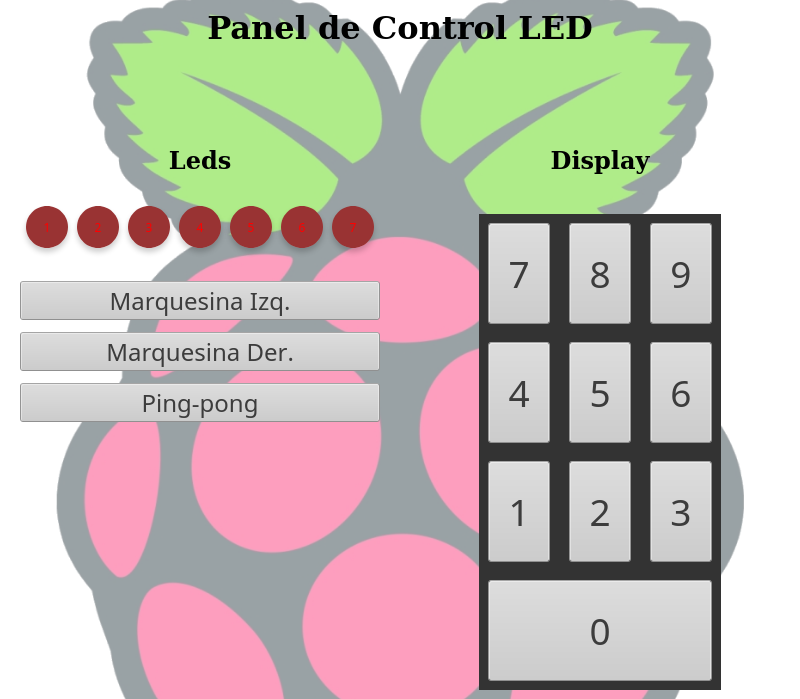
\includegraphics[height=7cm,keepaspectratio]{img/screenshot-ui.png}
	\caption{Caption: Intefaz de usuario del controlador de Leds en la Raspberry Pi.}
	\label{fig:hello-world} %CHKTEX 24
\end{figure}


\section{Experimentos}%
\label{sec:experiments}

Integre el código de la \prevpract{} en un archivo python llamado \texttt{led\_manager.py} y que ofrezca las siguientes funciones:
\begin{enumerate}
	\item{} [2 pts] Encendido del del 1--7 al presionar el boton adecuado
	\item{} [2 pts] Desplegado de la marquesina izquierda al presionar el boton adecuado
	\item{} [2 pts] Desplegado de la marquesina derecha al presionar el boton adecuado
	\item{} [2 pts] Desplegado de la marquesina tipo ping-pong al presionar el boton adecuado
	\item{} [2 pts] Desplegado del dígito correcto en el display de 7 segmentos al presionar el boton correspondiente
\end{enumerate}

Experimentos opcionales:
\begin{enumerate}
	\item{} [+2 pts] Modifique la implementación presentada para que sea posible definir la velocidad de rotación de la marquesina en la interfaz web.
	\item{} [+2 pts] Genere un único script de \emph{shell} (ej.~\emph{bash}) que automatice la configuración del punto de acceso inalámbrico.
	Dicho script recibirá dos parámetros opcionales: el SSID de la red y la contraseña a utilizar.
\end{enumerate}



\cleardoublepage
\appendix
\section{El archivo \texttt{webserver.py}}%
\label{sec:webserver-py}
\setlength{\columnsep}{1cm}
\begin{multicols}{2}
\lstinputlisting[%
	firstline=11,
	basicstyle=\scriptsize\ttfamily,
	xleftmargin=0cm,
	xrightmargin=0cm,
	frame=none,
	label=lst:webserver-py,
	caption=Archivo webserver.py
]{src/webserver.py}
\end{multicols}

\section{El archivo \texttt{user\_interface.html}}%
\label{sec:ui-html}
\setlength{\columnsep}{1cm}
\begin{multicols}{2}
\lstinputlisting[%
	basicstyle=\scriptsize\ttfamily,
	xleftmargin=0cm,
	xrightmargin=0cm,
	frame=none,
	label=lst:ui-py,
	caption=Archivo user\_interface.html,
]{src/user_interface.html}
\end{multicols}

\end{document}
